%%%%%%%%%%%%%%%%%%%%%%%%%%%%%%%%%%%%%%%%%%%%%%%%%%%%%%%%%%%%%%%%%%%%%%%
%%%%%%%%%%%%%%%%%%%%%%%%%%%%%%%%%%%%%%%%%%%%%%%%%%%%%%%%%%%%%%%%%%%%%%%
%%%%%                                                                 %
%%%%%     <file_name>.tex                                             %
%%%%%                                                                 %
%%%%% Author:      <author>                                           %
%%%%% Created:     <date>                                             %
%%%%% Description: <description>                                      %
%%%%%                                                                 %
%%%%%%%%%%%%%%%%%%%%%%%%%%%%%%%%%%%%%%%%%%%%%%%%%%%%%%%%%%%%%%%%%%%%%%%
%%%%%%%%%%%%%%%%%%%%%%%%%%%%%%%%%%%%%%%%%%%%%%%%%%%%%%%%%%%%%%%%%%%%%%%

%%%%%%%%%%%%%%%%%%%%%%%%%%%%%%%%%%%%%%%%%%%%%%%%%%%%%%%%%%%%%%%%%%%%%%%
%%%%%                                                                 %
%%%%%     Document Class                                              %
%%%%%                                                                 %
%%%%%%%%%%%%%%%%%%%%%%%%%%%%%%%%%%%%%%%%%%%%%%%%%%%%%%%%%%%%%%%%%%%%%%%
\documentclass[%
 oneside,      % Use the same margins for odd and even pages (cannot
               % be used with the 'twoside' option). 
% twoside,      % Use different margins for odd and even pages (cannot
               % be used with the 'oneside' option).
 openany,      % Open chapters on odd and even pages.
 halfparskip,  % Create small spaces for new paragraphs but no indents.
]{scrbook}

%%%%%%%%%%%%%%%%%%%%%%%%%%%%%%%%%%%%%%%%%%%%%%%%%%%%%%%%%%%%%%%%%%%%%%%
%%%%%                                                                 %
%%%%%     Preamble                                                    %
%%%%%                                                                 %
%%%%%%%%%%%%%%%%%%%%%%%%%%%%%%%%%%%%%%%%%%%%%%%%%%%%%%%%%%%%%%%%%%%%%%%
% Load the preamble from another file.
%%%%%%%%%%%%%%%%%%%%%%%%%%%%%%%%%%%%%%%%%%%%%%%%%%%%%%%%%%%%%%%%%%%%%%%
%%%%%%%%%%%%%%%%%%%%%%%%%%%%%%%%%%%%%%%%%%%%%%%%%%%%%%%%%%%%%%%%%%%%%%%
%%%%%                                                                 %
%%%%%     preamble.tex                                                %
%%%%%                                                                 %
%%%%% Author:      Michael Muehlberghuber                             %
%%%%% Created:     01.07.2012                                         %
%%%%% Description: This file contains the preamble of the             %
%%%%%              Semester-/Master-Project LaTeX report example.     %
%%%%%                                                                 %
%%%%% History:                                                        %
%%%%%%%%%%%%%%                                                        %
%%%%% 2012/07/01:  *) Created initial version.                        %
%%%%%                                                                 %
%%%%%%%%%%%%%%%%%%%%%%%%%%%%%%%%%%%%%%%%%%%%%%%%%%%%%%%%%%%%%%%%%%%%%%%
%%%%%%%%%%%%%%%%%%%%%%%%%%%%%%%%%%%%%%%%%%%%%%%%%%%%%%%%%%%%%%%%%%%%%%%

%%%%%%%%%%%%%%%%%%%%%%%%%%%%%%%%%%%%%%%%%%%%%%%%%%%%%%%%%%%%%%%%%%%%%%%
%%%%%                                                                 %
%%%%%     Package Loading                                             %
%%%%%                                                                 %
%%%%%%%%%%%%%%%%%%%%%%%%%%%%%%%%%%%%%%%%%%%%%%%%%%%%%%%%%%%%%%%%%%%%%%%

% Determines the input encoding.
\usepackage[%
 utf8,
% latin1
]{inputenc}

% ---------------------------------------------------------------------

% Determines the output encoding.
\usepackage[T1]{fontenc}

% ---------------------------------------------------------------------

% Code listing
\usepackage{listings}
\usepackage{float}
\usepackage{pgf}
\usepackage{siunitx}


% ---------------------------------------------------------------------

% Determines language settings.
\usepackage[%
 english    % You may change this to 'ngerman' in order to write a
            % german report.
]{babel}

% ---------------------------------------------------------------------

% Provides image loading.
\usepackage{graphicx}

% ---------------------------------------------------------------------

% Provides customization of chapter headings.
\usepackage[%
	Lenny     % Choose a nice layout for chapter headings.
]{fncychap}

% ---------------------------------------------------------------------

% Provides some blindtext.
\usepackage{lipsum}

% ---------------------------------------------------------------------

% Provides stretchable tables.
\usepackage{tabularx}

% ---------------------------------------------------------------------

% Provides some fancy boxes.
\usepackage{fancybox}

% ---------------------------------------------------------------------

% Provides subfigures.
\usepackage{subfig}

% ---------------------------------------------------------------------

% Provides colors in LaTeX.
\usepackage{xcolor}

% ---------------------------------------------------------------------

% Provides conditionals (for titlepage).
\usepackage{xifthen}

% ---------------------------------------------------------------------

% Provides the algorithm environment
\usepackage[ruled,%
            linesnumbered]{algorithm2e}

% ---------------------------------------------------------------------

% Provides bold greek math symbols.
\usepackage{bm}

% ---------------------------------------------------------------------

% Allows to include pdf documents.
\usepackage{pdfpages}

% ---------------------------------------------------------------------

% Provides nicer tables than the standard tables.
\usepackage{booktabs}

% ---------------------------------------------------------------------

% Provides simple line spacings.
\usepackage{setspace}

% ---------------------------------------------------------------------

% Provides simple line spacings.
\usepackage{geometry}

% ---------------------------------------------------------------------

% Provides more customizeable captions.
\usepackage{capt-of}

% ---------------------------------------------------------------------

% Provides small table of contents (e.g., for single chapters or the
% appendix).
\usepackage{minitoc}

% ---------------------------------------------------------------------

% Provides a simple command to describe a directory tree.
\usepackage{dirtree}

% ---------------------------------------------------------------------

%%%%%                                                             %%%%%
%%%%% ATTENTION: Loading further packagaes should go in here.     %%%%%
%%%%%                                                             %%%%%

% ---------------------------------------------------------------------

% Provides hyperlinks within your document. Should always be loaded at
% the end.
\usepackage{hyperref}

% ---------------------------------------------------------------------

% Provides multiple glossaries (incl. list acronyms, list of symbols,
% etc.).
\usepackage[%
 toc,              % Add the glossaries to the table of contents.
 acronym,          % Add a list of acronyms.
 acronymlists={hidden},
 section=chapter,  % Show glossary headers as chapters.
 nonumberlist,     % Do not print the page numbers next to glossary
                   % entries.
]{glossaries}



%%%%%%%%%%%%%%%%%%%%%%%%%%%%%%%%%%%%%%%%%%%%%%%%%%%%%%%%%%%%%%%%%%%%%%%
%%%%%                                                                 %
%%%%%     Custom Settings                                             %
%%%%%                                                                 %
%%%%%%%%%%%%%%%%%%%%%%%%%%%%%%%%%%%%%%%%%%%%%%%%%%%%%%%%%%%%%%%%%%%%%%%
% Do not use sans-serif fonts for all dispositions (chapters,
% sections, etc.)
\setkomafont{disposition}{\normalfont\bfseries}


%%%%%%%%%%%%%%%%%%%%%%%%%%%%%%%%%%%%%%%%%%%%%%%%%%%%%%%%%%%%%%%%%%%%%%%
%%%%%                                                                 %
%%%%%     Custom Macros                                               %
%%%%%                                                                 %
%%%%%%%%%%%%%%%%%%%%%%%%%%%%%%%%%%%%%%%%%%%%%%%%%%%%%%%%%%%%%%%%%%%%%%%
% Create an inline command for shell commands.
\newcommand{\shell}[1]{\texttt{#1}}

% Create an enviroment for a shell commands.
\newenvironment{shellenv}%
{\VerbatimEnvironment%
 \begin{Sbox}\begin{minipage}{0.97\textwidth}\begin{Verbatim}%
}%
{\end{Verbatim}\end{minipage}\end{Sbox}%
\setlength{\fboxsep}{6pt}\shadowbox{\TheSbox}}%

% Create an inline command for files.
\newcommand{\file}[1]{\texttt{#1}}

% Create a command for command parameters.
\newcommand{\parameter}[1]{$<$#1$>$}


%%%%%%%%%%%%%%%%%%%%%%%%%%%%%%%%%%%%%%%%%%%%%%%%%%%%%%%%%%%%%%%%%%%%%%%
%%%%%                                                                 %
%%%%%     Titlepage Macros - !!! DO NOT CHANGE !!!                    %
%%%%%                                                                 %
%%%%%%%%%%%%%%%%%%%%%%%%%%%%%%%%%%%%%%%%%%%%%%%%%%%%%%%%%%%%%%%%%%%%%%%
% Create a command for missing title page parameters.
\newcommand{\misspar}[1]{\textcolor{red}{\textbf{$<$#1$>$}}}

\makeatletter

% Redefine existing class macros as missing.
\title{\misspar{Specify Title}}%
\author{\misspar{Specify Author}}%
\date{\misspar{Specify Date}}%

% Define a command for setting the semester on the titlepage.
\def\@semester{\misspar{Specify Semester}}%
\newcommand{\setsemester}[1]{\def\@semester{#1}}%
\let\semester\setsemester%
\newcommand{\show@semester}{\@semester}%

% Define a command for setting the type of the report (Master Thesis,
% Semester Project, etc.) on the titlepage.
\def\@reporttype{\misspar{Specify Report Type}}%
\newcommand{\setreporttype}[1]{\def\@reporttype{#1}}%
\let\reporttype\setreporttype%
\newcommand{\show@reporttype}{\@reporttype}%

% Define a command for setting the image path for the image on the
% titlepage.
\def\@titlelogo{}%
\newcommand{\settitlelogo}[1]{\def\@titlelogo{#1}}%
\let\titlelogo\settitlelogo%

% Define a command for setting the image height on the titlepage.
\def\@logoheight{7cm}%
\newcommand{\setlogoheight}[1]{\def\@logoheight{#1}}%
\let\logoheight\setlogoheight%
\newcommand{\show@logoheight}{\@logoheight}%

% Define a command for setting the email on the titlepage.
\def\@email{\misspar{Specify E-Mail}}%
\newcommand{\setemail}[1]{\def\@email{#1}}%
\let\email\setemail%
\newcommand{\show@email}{\@email}%

% Define a command for setting the first supervisor on the titlepage.
\def\@firstsup{\misspar{Specify First Supervisor}}%
\newcommand{\setfirstsup}[1]{\def\@firstsup{#1}}%
\let\firstsup\setfirstsup%
\newcommand{\show@firstsup}{\@firstsup}%

% Define a command for setting the second supervisor on the titlepage.
\def\@secondsup{\misspar{Specify Second Supervisor}}%
\newcommand{\setsecondsup}[1]{\def\@secondsup{#1}}%
\let\secondsup\setsecondsup%
\newcommand{\show@secondsup}{\@secondsup}%

% Define a command for setting the professor on the titlepage.
\def\@professor{\misspar{Specify Professor}}%
\newcommand{\setprofessor}[1]{\def\@professor{#1}}%
\let\professor\setprofessor%
\newcommand{\show@professor}{\@professor}%

% Define a command for setting the margin on the title page.
\def\@titlepagemargin{3cm}%
\newcommand{\settitlepagemargin}[1]{\def\@titlepagemargin{#1}}%
\let\titlepagemargin\settitlepagemargin%
\newcommand{\show@titlepagemargin}{\@titlepagemargin}%

\makeatother


%%%%%
%%%%% Load the glossaries.
%%%%%
%%%%%%%%%%%%%%%%%%%%%%%%%%%%%%%%%%%%%%%%%%%%%%%%%%%%%%%%%%%%%%%%%%%%%%%
%%%%%                                                                 %
%%%%%     Make Glossaries                                             %
%%%%%                                                                 %
%%%%%%%%%%%%%%%%%%%%%%%%%%%%%%%%%%%%%%%%%%%%%%%%%%%%%%%%%%%%%%%%%%%%%%%

% Required to generate the index for the glossaries.
\makeglossaries

%%%%%%%%%%%%%%%%%%%%%%%%%%%%%%%%%%%%%%%%%%%%%%%%%%%%%%%%%%%%%%%%%%%%%%
%%%%%                                                                %
%%%%%     Definitions of all glossary entries which will appear in   %
%%%%%     the default (main) glossary.                               %
%%%%%                                                                %
%%%%%%%%%%%%%%%%%%%%%%%%%%%%%%%%%%%%%%%%%%%%%%%%%%%%%%%%%%%%%%%%%%%%%%

%\newglossaryentry{monkey}{name=Monkey,description={Lorem ipsum dolor
%sit amet, consetetur sadipscing elitr, sed diam nonumy eirmod tempor
%invidunt ut labore et dolore magna aliquyam erat, sed diam voluptua. At vero eos et accusam et justo duo dolores et ea
%rebum. Stet clita kasd gubergren, no sea takimata sanctus est Lorem
%ipsum dolor sit amet}}
\newglossaryentry{atomicOp}{name={Atomic Operations},
	description={An operation during which a processor can simultaneously read a location and write it in the same bus operation. This prevents any other processor or I/O device from writing or reading memory until the operation is complete.}
}


% Add all glossary entries to the glossary, even if they have not been
% referenced.
\glsaddall[types={main}]


%%%%%%%%%%%%%%%%%%%%%%%%%%%%%%%%%%%%%%%%%%%%%%%%%%%%%%%%%%%%%%%%%%%%%%
%%%%%                                                                %
%%%%%     Definitions of all acronyms which will appear in the list  %
%%%%%     of acronyms.                                               %
%%%%%                                                                %
%%%%%%%%%%%%%%%%%%%%%%%%%%%%%%%%%%%%%%%%%%%%%%%%%%%%%%%%%%%%%%%%%%%%%%

\newacronym[plural=APIs]{api} {API}{Application Programming Interface}
\newacronym[plural={CPUs}]{cpu} {CPU}{Central Processing Unit}
\newacronym{eees}{EEES}{Energy Efficient Embedded Systems}
\newacronym{iis} {IIS}{Integrated Systems Laboratory}
\newacronym[plural={ISAs}]{isa} {ISA}{Instruction Set Architecture}
\newacronym[plural={FPGAs}]{fpga}{FPGA}{Field Programmable Gate Array}
\newacronym{pcma}{PCMA}{Programmable Many Core Accelerator}
\newacronym{pulp}{PULP}{Parallel Ultra Low Power}
\newacronym{soc} {SoC}{System-on-Chip}
\newacronym{simd}{SIMD}{Single Instruction Multiple Data}
\newacronym{mit}{MIT}{Massachusetts Institute of Technology}
\newacronym[plural={ULPs}]{ulp}{ULP}{Ultra Low Power}
\newacronym{cuda}{CUDA}{Compute Unified Device Architecture}
\newacronym{opencl}{OpenCL}{Open Computing Language}
\newacronym{openmp}{OpenMP}{Open Multi-Processing}
\newacronym[plural={GPUs}]{gpu}{GPU}{Graphic Processing Unit}
\newacronym{eth}{ETH Zürich}{Eidgenössische Technische Hochschule Zürich}
\newacronym{llvm}{LLVM}{Low Level Virtual Machine}
\newacronym{mips}{MIPS}{Microprocessor without Interlocked Pipelined Stages}
\newacronym{aarch64}{AARCH64}{64 bit ARM architecture}
\newacronym{hero}{HERO}{Heterogeneous Embedded Research Platform}
\newacronym{rtl}{RTL}{Register Transfert Level}
\newacronym{ci}{CI}{Continuous Integration}



% Add all acronyms to the list of acronyms even if they have not been
% referenced.
\glsaddall[types={\acronymtype}]


% Define which source files should actually been processed.
%\includeonly{./content/06-design_implementation}


%%%%%%%%%%%%%%%%%%%%%%%%%%%%%%%%%%%%%%%%%%%%%%%%%%%%%%%%%%%%%%%%%%%%%%%
%%%%%                                                                 %
%%%%%     Document Settings                                           %
%%%%%                                                                 %
%%%%%%%%%%%%%%%%%%%%%%%%%%%%%%%%%%%%%%%%%%%%%%%%%%%%%%%%%%%%%%%%%%%%%%%

%%%%% Mandatory title page settings.
\title{\LaTeX{} Report Template}
\author{Pierre-Hugues BLELLY}
\email{pblelly@student.ethz.ch}
\date{May 2020}
\semester{Spring Semester 2020}
\reporttype{Semester Project / Master Project}
\firstsup{Matheus Cavalcante, matheusd@iis.ee.ethz.ch}
\secondsup{Samuel Riedel, sriedel@student.ethz.ch}
\professor{Prof. Luca Benini, lbenini@ethz.ch}

%%%%% Optional title page settings.
\titlelogo{./figures/titlepage_logo}  % Title page logo path.
\logoheight{7cm}                      % Height of the title page logo.
\titlepagemargin{3cm}                 % Margin on the title page.


%%%%%%%%%%%%%%%%%%%%%%%%%%%%%%%%%%%%%%%%%%%%%%%%%%%%%%%%%%%%%%%%%%%%%%%
%%%%%                                                                 %
%%%%%     Start of Document                                           %
%%%%%                                                                 %
%%%%%%%%%%%%%%%%%%%%%%%%%%%%%%%%%%%%%%%%%%%%%%%%%%%%%%%%%%%%%%%%%%%%%%%
\begin{document}

% Prepare document for minitoc insertions.
\dominitoc

\frontmatter

% Create title.
%%%%%%%%%%%%%%%%%%%%%%%%%%%%%%%%%%%%%%%%%%%%%%%%%%%%%%%%%%%%%%%%%%%%%%%
%%%%%%%%%%%%%%%%%%%%%%%%%%%%%%%%%%%%%%%%%%%%%%%%%%%%%%%%%%%%%%%%%%%%%%%
%%%%%                                                                 %
%%%%%     <file_name>.tex                                             %
%%%%%                                                                 %
%%%%% Author:      <author>                                           %
%%%%% Created:     <date>                                             %
%%%%% Description: <description>                                      %
%%%%%                                                                 %
%%%%%%%%%%%%%%%%%%%%%%%%%%%%%%%%%%%%%%%%%%%%%%%%%%%%%%%%%%%%%%%%%%%%%%%
%%%%%%%%%%%%%%%%%%%%%%%%%%%%%%%%%%%%%%%%%%%%%%%%%%%%%%%%%%%%%%%%%%%%%%%
\makeatletter
\newgeometry{margin = \@titlepagemargin}
\begin{titlepage}

 % Remove the page number in the footer.
 \thispagestyle{empty}

 \begin{center}
  \begin{minipage}[b]{0.45\linewidth}
   \vspace{0pt}	
   \includegraphics[width=0.8\linewidth]{./figures/eth_logo}
  \end{minipage}\hfill
  \begin{minipage}{0.45\textwidth}
%   \vspace{-1cm}\flushright{Institut f\"ur Integrierte Systeme\\Integrated Systems Laboratory}
   \vspace{-0.55cm}\flushright{\fontfamily{let}\fontseries{b}\fontsize{\@xpt}{18}\selectfont Institut f\"ur Integrierte Systeme\\Integrated Systems Laboratory}
  \end{minipage}

  \vspace{0.1cm}

  \hspace*{0.15cm}\rule{0.985\textwidth}{0.4pt}

  \vspace{0.5cm}

  {\Large\textsc{Department of Information Technology and \\Electrical Engineering}}

  \vspace{0.2cm}

  \show@semester

  \vfill

  \begin{spacing}{2.0}
  {\Huge\textbf{\@title}}
  \end{spacing}

  \vspace{0.2cm}

  \show@reporttype

  \vfill
  
  \ifx\@titlelogo\@empty
   \relax
  \else
   \includegraphics[height = \@logoheight]{\@titlelogo}
  \fi
    
  \vfill

  {\Large \@author}\\
  {\@email}
  
  \vfill
  
  \@date

  \vfill
  
  \begin{tabular}{ll}
   Supervisors: & \show@firstsup \\
                & \show@secondsup \\
   \rule{0pt}{3ex}Professor: & \show@professor \\
  \end{tabular}

 \end{center}
\end{titlepage}
\restoregeometry
\makeatother

%\maketitle

% Include acknowledgements, abstract, etc...
%%%%%%%%%%%%%%%%%%%%%%%%%%%%%%%%%%%%%%%%%%%%%%%%%%%%%%%%%%%%%%%%%%%%%%%
%%%%%%%%%%%%%%%%%%%%%%%%%%%%%%%%%%%%%%%%%%%%%%%%%%%%%%%%%%%%%%%%%%%%%%%
%%%%%                                                                 %
%%%%%     <file_name>.tex                                             %
%%%%%                                                                 %
%%%%% Author:      <author>                                           %
%%%%% Created:     <date>                                             %
%%%%% Description: <description>                                      %
%%%%%                                                                 %
%%%%%%%%%%%%%%%%%%%%%%%%%%%%%%%%%%%%%%%%%%%%%%%%%%%%%%%%%%%%%%%%%%%%%%%
%%%%%%%%%%%%%%%%%%%%%%%%%%%%%%%%%%%%%%%%%%%%%%%%%%%%%%%%%%%%%%%%%%%%%%%

\chapter*{Acknowledgements}
Ceci est un test de mon script

%%%%%%%%%%%%%%%%%%%%%%%%%%%%%%%%%%%%%%%%%%%%%%%%%%%%%%%%%%%%%%%%%%%%%%%
%%%%%%%%%%%%%%%%%%%%%%%%%%%%%%%%%%%%%%%%%%%%%%%%%%%%%%%%%%%%%%%%%%%%%%%
%%%%%                                                                 %
%%%%%     <file_name>.tex                                             %
%%%%%                                                                 %
%%%%% Author:      <author>                                           %
%%%%% Created:     <date>                                             %
%%%%% Description: <description>                                      %
%%%%%                                                                 %
%%%%%%%%%%%%%%%%%%%%%%%%%%%%%%%%%%%%%%%%%%%%%%%%%%%%%%%%%%%%%%%%%%%%%%%
%%%%%%%%%%%%%%%%%%%%%%%%%%%%%%%%%%%%%%%%%%%%%%%%%%%%%%%%%%%%%%%%%%%%%%%

\chapter*{Abstract}
\lipsum[1-2]

%%%%%%%%%%%%%%%%%%%%%%%%%%%%%%%%%%%%%%%%%%%%%%%%%%%%%%%%%%%%%%%%%%%%%%%
%%%%%%%%%%%%%%%%%%%%%%%%%%%%%%%%%%%%%%%%%%%%%%%%%%%%%%%%%%%%%%%%%%%%%%%
%%%%%                                                                 %
%%%%%     <file_name>.tex                                             %
%%%%%                                                                 %
%%%%% Author:      <author>                                           %
%%%%% Created:     <date>                                             %
%%%%% Description: <description>                                      %
%%%%%                                                                 %
%%%%%%%%%%%%%%%%%%%%%%%%%%%%%%%%%%%%%%%%%%%%%%%%%%%%%%%%%%%%%%%%%%%%%%%
%%%%%%%%%%%%%%%%%%%%%%%%%%%%%%%%%%%%%%%%%%%%%%%%%%%%%%%%%%%%%%%%%%%%%%%
\makeatletter
\chapter*{Declaration of Originality}
I hereby confirm that I am the sole author of the written work here
enclosed and that I have compiled it in my own words. Parts excepted
are corrections of form and content by the supervisor. For a detailed
version of the declaration of originality, please refer to
Appendix~\ref{chap:originality}
\\
\\
\\
\\
\@author,\\
Zurich, \@date\\



% Insert table of contents, list of figures, and list of tables.
\tableofcontents
\listoffigures
\listoftables

% Print list of acronyms.
\setlength{\glslistdottedwidth}{0.2\linewidth}
\printglossary[type=\acronymtype,style=listdotted,title=List of Acronyms]


%%%%%
%%%%% Start the actual main content part.
%%%%%
\mainmatter

% Include the actual content files.
%%%%%%%%%%%%%%%%%%%%%%%%%%%%%%%%%%%%%%%%%%%%%%%%%%%%%%%%%%%%%%%%%%%%%%%
%%%%%%%%%%%%%%%%%%%%%%%%%%%%%%%%%%%%%%%%%%%%%%%%%%%%%%%%%%%%%%%%%%%%%%%
%%%%%                                                                 %
%%%%%     <file_name>.tex                                             %
%%%%%                                                                 %
%%%%% Author:      <author>                                           %
%%%%% Created:     <date>                                             %
%%%%% Description: <description>                                      %
%%%%%                                                                 %
%%%%%%%%%%%%%%%%%%%%%%%%%%%%%%%%%%%%%%%%%%%%%%%%%%%%%%%%%%%%%%%%%%%%%%%
%%%%%%%%%%%%%%%%%%%%%%%%%%%%%%%%%%%%%%%%%%%%%%%%%%%%%%%%%%%%%%%%%%%%%%%

\chapter{Introduction}

    Thanks to the smaller nodes of modern lithography technologies and the transistor density we can achieve with them, modern low-power \glspl{cpu} can have a large amount of cores while keeping their power consumption under a few Watts. A single Raspberry Pi 3 has a peak performance of 6 \si{gflop/s} for a power consumption of only 7 Watts~\cite{Art:RpiClusters}.
    Embedded systems can take advantage of this increase in efficiency to become more autonomous and not rely on an external computer for heavy computation. We can find this type of architecture on some nano drones such as the CrazyFlie 2.0~\cite{Web:CrazyFlie20}, which can be extended with additional shields. Using a custom shield, the \gls{iis} of \gls{eth} achieved to analyze in real-time a video signal and train a neural network for autonomous navigation~\cite{Art:NanoDrone}. The compute unit achieved a rate of 281 \si{MMAC/s} on a power-enveloppe of only 45 \si{mW}.

    To improve the energy efficiency and the computing power of \gls{ulp} systems, new architectures are needed. To keep the power consumption low, an embedded system needs to power it's subsystems only when needed. The CrazyFlie uses a low power ARM Cortex-M4 to manage the flight of the drone, and can power on and of it's extension board as needed. The shield use a \gls{pulp} cluster, which is an \gls{riscv} \gls{soc} which can be configured with up to eight cores. With this configuration, the energy consumption of the CrazyFlie stays low, as most of the time it only uses the micro controller to flight and only power on the shield for the heavy computation.

	Heterogeneous systems are composed of multiple coprocessors all managed by a host processor. This architecture is interesting when it comes to embedded systems, as it is possible to achive greater energy efficiency than homogeneous systems. If each coprocessor has been designed to solve a certain task, it can achieve energy efficiency than a general purpose \gls{cpu}. 
	In this article~\cite{Art:Harnessing} pusblished by the University of California,  researchers showed that under heavy design constraints (such as die area or therman dissipation), systems using multiple \glspl{isa} achieved better performances than their best homogeneous counterpart.

This strategy has been used in the \gls{soc} industry by ARM since 2011~\cite{Art:bigLITTLE}. The  big.LITTLE architecture is based on two clusters of ARM Cortex A7(the ``LITTLE''cores) and A15 (the ``big'' cores), and was designed to increase the computing power in low power systems such as smartphones while increasing the battery life of the device. This architecture relied on a single~ \gls{isa}(ARMv7). The goal was to use the more powerful cores during heavy computation or graphic rendering, and let the low power cores handle the background tasks or manage the device during sleep.
	Presently, every smartphone \gls{soc} manufacturer use the bigLITTLE architecture or a similar technology.


Even in data centers, where power consumption is also an issue, \glspl{gpu} are used thanks to their massive core count and the various \glspl{api} such as \gls{cuda} or \gls{opencl} which simplify the developement process for \gls{gpu} accelerators.

    \gls{hero}~\cite{Art:Hero} is a heterogeneous system developed by the \gls{iis} of \acrshort{eth} and the \gls{eees} of the University of Bologna.
	This platform is composed of a hard macro ARM 64 \gls{cpu} and up to eight \gls{pulp} clusters(\gls{riscv} cores) running on an Xilinx ZYNC ZC706 \gls{fpga}.

    This platform is designed to ``facilitate rapid exploration on all software and hardware layers''~\cite{Art:Hero}, and includes a heterogeneous compilation toolchain with support for \gls{openmp}, an \gls{api} developed to make developement of multi threaded applications easier~\cite{Web:Wikipedia_OpenMP}. This \gls{api} implements new preprocessor instructions to tell the compiler how to execute the code on the system.



\section {Design Issue with heterogeneous systems}

    During their conception, numerous design choices need to be made specifically how the \glspl{cpu} in the system will interact will each other. These choices will impact the peak performance of the design or its power consumption~\cite{Art:Harnessing}. The computer architect has to choose how the different \glspl{pcma} will interact, how they will share data, maybe extend the existing \glspl{isa} to distribute tasks, and so on.
    The software design is challenging, when compiling for heterogeneous platforms. The compiler needs to create an executable that will run on the host processor, but also dedicate parts of the final binary to embed the code that will be distributed on the \glspl{pcma}.
	Code distribution is handled by the programmer, \glspl{api} such as \gls{cuda}, \gls{opencl} or \gls{openmp} using function calls tell the compiler how to execute the code and on which \gls{pcma}. 
	Even though these \gls{api} did a great job at making the overall developpement easier, most of the work is still done by hand. The programmer has to handle memory mapping (will the data be stored on the host or the \gls{pcma} memory), every task needs to be scheduled by hand, and distributed on the correct \gls{pcma}. 
	Moreover, the code is often not portable as some schedule are target dependant. An algorithm coded with \gls{cuda} will only run on a \gls{gpu}, so the code can't be reused for another platform.
	Porting \gls{api} to new platform is not trivial, and require sometime months of work, to make the \gls{api} run on the new target.





\section {Currently Available Workflow for \acrshort{hero}}
    Currently, \gls{hero} supports \gls{openmp}~\cite{Report:SoftwareStack}, an \gls{api} which ``defines a portable, scalable model with a simple and flexible interface for developing parallel applications on platforms from the desktop to the supercomputer''~\cite{Web:OpenMp}. 
	This \gls{api} has been implemented on \gls{hero} to easily take advantage of the \gls{pulp} clusters. The toolchain uses the Clang compiler~\cite{Web:Wikipedia_OpenMP} to compile the applications. \gls{hero} uses custom Clang front ends to supports all the available configurations (only the \gls{pulp} cluster for simulation with the ARM host \gls{cpu} or with a 64 bits \gls{riscv} \gls{cpu}).

    To distribute the code, \gls{openmp} uses preprocessor instructions to tell Clang where the code will run and how it will be executed. Exploring the design space using \gls{openmp}'s directive can be time-consuming. For example, the developer must explicitly tell which part of the code to offload. Trying to change the order of multiple loops may cause bugs in the algorithmn, and complex schedules often impact code readability making them harder to debug

    Halide~\cite{Art:Halide} was proposed to explore the idea of separating the algorithm from how the code will be executed on the target(the schedule).
    This separation makes testing different schedule easier on the developer, as the algorithm code will stay the same, and only the scheduling will be changed when testing.
    Every processing pipeline designed with Halide has two parts. The first part consists of the functional description of the processing kernel, i.e. the algorithm that will be executed. 
	The second part is the schedule of the pipeline. The programer will explicitely tell Halide how the pipeline should be executed. Thanks to specific function calls, the developer can decide whether the code will be run on multiple threads or a single one, change the order of execution of different parts, split loops, unrolls them. The developer can still have the freedom to implement any schedule he wants but without having to change the main algorithm.
    This programming model is interesting because the developer can quicky implement the algorithm without having to take into account the boundaries of the inputs, and then work on an optimal schedule, or quickly adapt it if the algorithm need to be executed on another platform.

    The intermediate variables can be bounded afterwards if needed, and the pricipal variables such as characteristics of the inputs are automatically bounded by Halide. An image processing pipeline will only compute the output on the pixels of the input.
    The scheduling process can even be done automatically during the compilation by the library, in order to find an optimal schedule on the target platform.

%%%%%%%%% GOAL OF THE PROJECT
	The goal of this project was to port Halide to \gls{hero}, and execute image processing kernels on the \gls{hero} system running on an \gls{fpga}. First Halide needs to be compiled to support \gls{riscv} and compile basic applications to the hardware simulation. From then we can work on the heterogeneous compilation to support the current \gls{hero} test platform.

%%% Local Variables: 
%%% mode: latex
%%% TeX-master: "../report_template"
%%% End: 

%%%%%%%%%%%%%%%%%%%%%%%%%%%%%%%%%%%%%%%%%%%%%%%%%%%%%%%%%%%%%%%%%%%%%%%
%%%%%%%%%%%%%%%%%%%%%%%%%%%%%%%%%%%%%%%%%%%%%%%%%%%%%%%%%%%%%%%%%%%%%%%
%%%%%                                                                 %
%%%%%     <file_name>.tex                                             %
%%%%%                                                                 %
%%%%% Author:      <author>                                           %
%%%%% Created:     <date>                                             %
%%%%% Description: <description>                                      %
%%%%%                                                                 %
%%%%%%%%%%%%%%%%%%%%%%%%%%%%%%%%%%%%%%%%%%%%%%%%%%%%%%%%%%%%%%%%%%%%%%%
%%%%%%%%%%%%%%%%%%%%%%%%%%%%%%%%%%%%%%%%%%%%%%%%%%%%%%%%%%%%%%%%%%%%%%%

\chapter{Preliminaries / Background}
\section{Hero}

\section{Halide Language}
	\subsection { Programing model}
		Halide is a functionnal program embedded into C++ designed to write high performance image and array processing code \cite{Web:Halide}. This language uses a functionnal paradigm to describe the functionnalities of the pipeline. The scheduling of the pipeline is described separately, which allow the developper to explore a wide range of schedule without having to rewrite most of the code. 
		Every pipeline is a function (\verb|Halide::Func| composed of other functions and expressions (\verb|Halide:expr|). These two objects  use special variables (\verb|Halide:Vars|) to describe the operation executed on the array. The code snippet 
		\ref{code:simple_pipeline} 
		describe a basic pipeline which compute the distance of each coordinate of the array from on position specified by the vector \verb|(center_x, center_y)|.


\lstset{basicstyle=\ttfamily\footnotesize,breaklines=true,tabsize=2}
\begin{lstlisting}[caption={Simple Pipeline Example}, captionpos=b, label={code:simple_pipeline}]
Halide::Var x, y;
Halide::Param center_x, center_y;
Halide::Expr offset = Halide::pow(x - center_x, 2) 
                      + Halide::pow(y - center_y, 2);

	gradient(x, y) = offset;
\end{lstlisting}

	After designing the  pipeline, we can define it's schedule via the different directive included in Halide. Halide implements all the basic scheduling option like parallelizing, unrolling, splitting ... These options will be described in the section 
	\nameref{section:scheduling}
	. The snippet 
	\ref{code:simple_pipeline_schedule} 
	shows a simple schedule applied on our gradient. This schedule consists of parallelizing the execution over the \texttt{x} axis, and unrolling along the  \texttt{y} axis.

	\begin{lstlisting}[caption={Simple Pipeline Example}, captionpos=b,label={code:simple_pipeline_schedule}];
	gradient.parallel(x);
	gradient.unroll(y, 10);
	\end{lstlisting}


	To execute our pipeline, Halide provides a large range of options, we can execute it directly using the \verb|.realize(x_max, y_max)| directive, this will execute the pipeline on a rectangle starting from it's top left corner in  \verb|(0,0)| to it's bottom right corner in \verb|(x_max, y_max)|.
	
	But Halide also gives the programmer a lot off options to execute the pipeline, it's able to convert the code to C code, llvm assembly file, or already compiled object file specific to a given target. More over, Halide support a wire variety of CPU architecture (X86, ARM, MIPS, PowerPc, Risc-V  ), operating systems ( Linux, Windows, Android, Mac) and also Gpu Api's (Cuda, OpenCL, OpenGl, DirectX ...). Halide support for new architecture is getting better and better, and is by design targeted for cross compilation and Heterogeneous systems.

	\subsection{Debugging Options}

	\subsection {Basic Scheduling Options}
	\label{section:scheduling}
	Halide implement different scheduling instruction, and most of them aren't architecture specific. 
	\subsubsection{Non Architecture Specific Instrutions}
	\begin{itemize}
		\item Reorder : Tells halide how to traverse the domain of the pipeline stage (ffor example in a column major or row major way)
		\item Split   : Split a dimension along inner and outer subdimensions.
		\item Tile    : Cut the domain in tiles.
		\item Fuse    : Join two dimensions in a single fused dimension.
		\item Unroll  : Unroll along one dimension.
	\end{itemize}

	Some of the primitives such as vectorize or parallel. needs to be implemented on the target platform as they take advantage of the specificities of the system. To do so Halide uses some functions which are defined in a header file we can get when compiling the pipeline.

	\subsection { Porting Halide to new Platforms}
		From the header file, we can find the functions vital for halide to work and implement them in the pulp runtime. From then, we have to compile the pipeline to a risc-V object file, and then compile the main application using this object file and the provided header. When we will compile the final application using the hero toolchain, the linker will link the halide function calls to the implemented functions in the pulp runtime.
		Currently, only the memory allocation, print, and fork primitive are implemented but they are sufficient to try some basic parallel schdeules.

\section{Compilation Workflow}
	Hero currently have different platforms, and also different workflow. I started by working on the simulation platform which simulate an eight-core pulp cluster. Then I tried to port it to the hardware platform (One hard ARM core and a PULP cluster implemented on the FPGA). The compilation is slightly different for both platform, so I started by working on the simulation platform which is not heterogeneous.
\section{Simulation}
	The compilation process for the simulation platform is quite easy,  we start by compiling the C++ code which will generate the final pipeline, we then run this application, to generate the pipeline and the matching header file.
	Then we compile the true application which will call the pipeline. During the process, we add the object file of the pipeline in the source file, g++ will then link the pipeline with the main application and also the halide calls to the pulp runtime functions.
		
\section{The full hero platform}
	The hardware platform has a more complex compiling process, currently, the applications use OpenMp to distribute the code to the pulp cluster. With instructions such as \verb| #pragma omp target device(BIGPULP_MEMCPY) | to  explicitely tell the compiler to distribute the following part of the code to the pulp cluster. The application is compiled using Clang and a the clang-offlad bundler to create an heterogeneous application that will run on both platform.

%%% Local Variables: 
%%% mode: latex
%%% TeX-master: "../report_template"
%%% End: 

%%%%%%%%%%%%%%%%%%%%%%%%%%%%%%%%%%%%%%%%%%%%%%%%%%%%%%%%%%%%%%%%%%%%%%%
%%%%%%%%%%%%%%%%%%%%%%%%%%%%%%%%%%%%%%%%%%%%%%%%%%%%%%%%%%%%%%%%%%%%%%%
%%%%%                                                                 %
%%%%%     <file_name>.tex                                             %
%%%%%                                                                 %
%%%%% Author:      <author>                                           %
%%%%% Created:     <date>                                             %
%%%%% Description: <description>                                      %
%%%%%                                                                 %
%%%%%%%%%%%%%%%%%%%%%%%%%%%%%%%%%%%%%%%%%%%%%%%%%%%%%%%%%%%%%%%%%%%%%%%
%%%%%%%%%%%%%%%%%%%%%%%%%%%%%%%%%%%%%%%%%%%%%%%%%%%%%%%%%%%%%%%%%%%%%%%

\chapter{Design Implementation}


\section { Porting Halide to new targets}
    Halide programs relies on the \gls{llvm} libraries to compile code for the desired targets. To build the Halide library, we first need to build \gls{llvm} with the correct flags and add the support for the building machine.
    As the \gls{hero} toolchain already has a build of this compiler, we can use it to compile Halide, but the \texttt{-DBUILD\_SHARED\_LIBS} flag has to be disabled, as Halide does not support shared libraries.
    We added a \texttt{make} target to main \texttt{Makefile} of the project, to simplify the installation process.

    Once the installation process was complete, we worked on porting Halide to \gls{hero} on the hardware simulation. This was the first step of the project, as this platform is easier to work with than the full \gls{hero} platform. We do not have to work with the heterogeneous toolchain, so the compilation process is simpler.
    Unlike the hardware platform, the hardware simulator only simulate a single  \gls{pulp} cluster configured with eight cores.
    The first core of the cluster acts as the host, it first initializes the cluster and then starts the execution of the application.
     When a fork is executed on the other cores, the host core continues the execution like the other cores.
     

    %%%%%%%%%%%%%
    \section{Compilation Workflow}

\begin{figure}[H]
\dirtree{%
    .1 halide-examples/.
    .2 common/.
    .3 defaultHalide.mk.
    .2 myApp/.
    .3 main.c.
    .3 Makefile.
    .3 lib/.
    .4 halidePipeline.cpp.
    }
    \caption{Directory structure for Halide applications.}
    \label{Fig:DirectoryStructure}
\end{figure}



    Every application follows the directory structure described in Figure~\ref{Fig:DirectoryStructure}, the \texttt{common} folder is shared between all the applications and contains a common \texttt{Makefile} that will be included in every application's \texttt{Makefile}.
    The source code is split between two files, the pipeline generator in the \texttt{lib/} folder, and the main \gls{hero} application.
    The pipeline generator uses Halide to generate the pipeline object file which will be linked during the compilation of the application.

\begin{figure}[h]
    \centering
    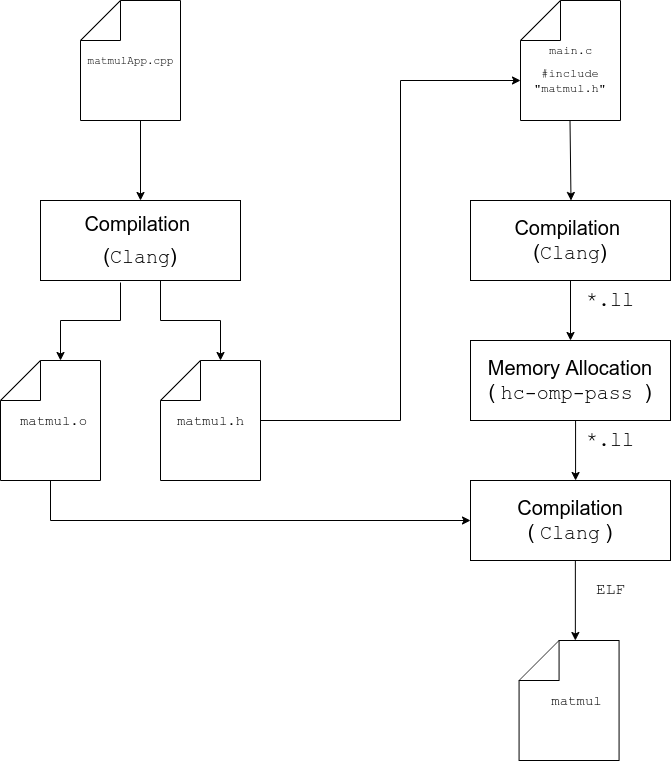
\includegraphics[width=.7\textwidth]{./figures_raw/compilationWorkflow.png}
    \caption{Compilation Workflow for an Halide Application.}
    \label{fig:compwork}
\end{figure}

    Figure~\ref{fig:compwork} shows the whole compilation process to build a Halide application for \gls{hero}.
    The compilation is done in two steps. First, we compile the Halide program to execute on the build computer.
    This program is then run on the machine and creates a RISC-V object file and a header file.
    This header file must be included in the \gls{hero} application (\texttt{main.c}).
    The application building process is based on the \gls{openmp} workflow, we used the same \texttt{Makefile} with some modification to link the pipeline with the main application. 

    We first compile the source code to \gls{llvm} assembly code. Then due to the heterogeneous nature of the system, a custom program: \texttt{hc-omp-pass}, changes every part of the code that may cause issue due to architectural differences between the host and the \gls{pcma} (on \gls{hero}v3, the host can be a 64-bit RISC-V or an ARM processor, and the pointers have to be changed due to the incompatibilities between the 32-bit and 64-bit addressing).
    In our case, as we only compile for the \gls{pulp} cluster, this step does not affect the code, but it will be useful to support the full \gls{hero} platform. 
    Then, we use the \gls{llvm} assembly files coupled with the pipeline object file to generate the final binary.


    The header file generated by Halide declares every function available on Halide and required to have a fully working Halide implementation. 
    Most of them do not use platform-specific functionalities, and will be compiled to RISC-V without any issue.
    But others such as memory management functions or thread distribution functions, which require dedicated functions in the \gls{pulp} runtime have to be overwritten to work on the cluster.
    Finally, functions that are only called when using the Just in Time compilation or other advanced functionalities, have to be overwritten, but we can implement simple stub functions to prevent linking errors, as we do not need those functionalities for our pipelines. 
    The comments in the header precisely describes the role of each function and under which circumstances they have to be overwritten.
    We implemented the necessary functions in the \gls{pulp} runtime to make the parallel schedule work, as this schedule is essential to take advantage of the high core count of the cluster.
 
\section{Schedule Implementation }
    Most schedules work out of the box, because they do not need to access any runtime specific function.
    Halide generates them by altering the source code as operations such as splitting and unrolling are just modification of the loops of the pipeline. 
    Even the vectorize schedule does not need any specific instructions, Halide will rewrite the schedule as if the pipeline was manipulating a vector even if the hardware target does not support \gls{simd} instructions.
     To use this schedule fully,  a hardware specific modification would be needed.
    Memory access and thread task distribution on the cluster have to be overwritten as they use specific runtime functions.

    \subsection{Modification to the PULP runtime}

    The missing Halide functions need to be accessible to the \gls{pulp} runtime. To do so, we created a new file in the \gls{pulp} runtime (\texttt{halide\_api.c}). 
    This file contains all the \gls{api} functions required to run Halide on \gls{hero}.

\begin{lstlisting}[language=C,caption={The \texttt{halide\_do\_par\_for} function.},label={lst:halidedoparfor},captionpos=b]
int halide_do_par_for(void *user_context,halide_task_t task,
    int min, int size, uint8_t *closure) {
    // Mount the cluster
    rt_cluster_mount(1, 0, 0, NULL);

    unsigned arguments[4];
    arguments[0] = (unsigned)user_context;
    arguments[1] = (unsigned)size;
    arguments[2] = (unsigned)closure;
    arguments[3] = (unsigned)task;

    // Dispatch the task to the cluster
    rt_team_fork(0, pulp_do_halide_par_for_fork, arguments);

    // Unmount the cluster
    rt_cluster_mount(0, 0, 0, NULL);

    return 0;
}
\end{lstlisting}


    The Listing~\ref{lst:halidedoparfor} shows the full source code of the \texttt{halide\_do\_par\_for} function.
    This function is only called once during the execution of a parallel schedule. On the hardware simulator, only the first core of the cluster executes it.
    The \texttt{size} argument of the function determines the number of threads to create, and will be used by the cores to determine which task to execute. 
    This function creates the thread pool for the parallel execution of the pipeline. As \gls{hero} does not have a standard way of managing threads, we had to overwrite this function.
    The \texttt{rt\_cluster\_mount} is called to prepare the cluster before distributing the tasks.
    The \texttt{argument} structure packs all the data about the tasks: the user context,  the number of threads, and the starting point of the execution.
    \texttt{rt\_team\_fork} will then create a team of workers which will all execute the same function: \texttt{halide\_do\_par\_for\_fork}.
    The first argument of \texttt{rt\_team\_fork} indicates how many fork the cluster will do, if it is set to zero, the cluster will reuse the last number of threads (which is by default eight).



\begin{lstlisting}[language=C,caption={The \texttt{halide\_do\_par\_for\_fork} function.},label={lst:halidedoparforfork},captionpos=b]
void pulp_do_halide_par_for_fork(void *arg) {
  unsigned *arguments = (unsigned *)arg;

  void *user_context = (void *)arguments[0];
  unsigned task_num = arguments[1];
  uint8_t *closure = (uint8_t *)arguments[2];
  halide_task_t task = (halide_task_t)arguments[3];

  for (unsigned core_id = rt_core_id(); core_id < task_num; core_id += (int)&__rt_nb_pe) {
    task(user_context, core_id, closure);
  }

}
\end{lstlisting}
    The source code of this function is shown in listing~\ref{lst:halidedoparforfork}, every worker iterates over the task queue, and executes only the task they have been assigned.
    The assignment is done by comparing the task identifier with the worker's core identifier, if \texttt{core\_id = task\_id \% nb\_cores}, then the task will be executed by the worker. 
	The first core then wait for all workers to complete before shutting turning off the cluster and continuing the excution of the application.


%% Pros and cons of such a distribution scheme
    
    This distribution scheme has the advantage of being easy to implement and splitting the task is done in a way that facilitates debugging if needed.
    But, it can't adapt if one core is delayed or its task takes longer to compute.
So if one core has to execute some tasks which are two or three times longer to execute, all the other core will wait for this core to compile.
    It may be interesting to dynamically reschedule the tasks depending on the free cores.


%%%%%%%%%%%%%%%%%%%%%%%%%%%%%%%%%%%%%%%%%%%%%%%%%%%%%%%%%%%%%%%%%%%%%%%
%%%%%%%%%%%%%%%%%%%%%%%%%%%%%%%%%%%%%%%%%%%%%%%%%%%%%%%%%%%%%%%%%%%%%%%
%%%%%                                                                 %
%%%%%     <file_name>.tex                                             %
%%%%%                                                                 %
%%%%% Author:      <author>                                           %
%%%%% Created:     <date>                                             %
%%%%% Description: <description>                                      %
%%%%%                                                                 %
%%%%%%%%%%%%%%%%%%%%%%%%%%%%%%%%%%%%%%%%%%%%%%%%%%%%%%%%%%%%%%%%%%%%%%%
%%%%%%%%%%%%%%%%%%%%%%%%%%%%%%%%%%%%%%%%%%%%%%%%%%%%%%%%%%%%%%%%%%%%%%%

\chapter{Results}
\section{Test Setup}
	I benchmarked two applications on two platforms. I benchmarked the halide port  on the hardware simulation for the PULP cluste, and one openMp matrix multiplication application on the developpement platform on a Xilinx ZCU102. For both application, I generated random matrices of différent sizes, and for each sizes multiplication I counted the number of cycles needed to complete the operation. 
	With this setup, we can easily compare the performances of halide and OpenMp in a real world scenario for at least two basic schedules: Single threaded and Multi Threaded.
	To give the results a more meaning I also calculated the number of operations per cycles where one operation can either be an addition a multiplication or a memory access (which take 2 cycles each), so for a matrix of size n, the number of operations to finish the multiplication is : $6 * n ** 3 + n ** 2$ (each coefficient needs $2n$ memory accesses, $2n$ additions and multiplications and one memory store).

\section{Comparaison between OpenMp and Halide on the different platforms}

%%%%%%%%%%%%%%%%%%%%%%%%%%%%%%%%%%%%%%%%%%%%%%%%%%%%%%%%%%%%%%%%%%%%%%%
%%%%%%%%%%%%%%%%%%%%%%%%%%%%%%%%%%%%%%%%%%%%%%%%%%%%%%%%%%%%%%%%%%%%%%%
%%%%%                                                                 %
%%%%%     <file_name>.tex                                             %
%%%%%                                                                 %
%%%%% Author:      <author>                                           %
%%%%% Created:     <date>                                             %
%%%%% Description: <description>                                      %
%%%%%                                                                 %
%%%%%%%%%%%%%%%%%%%%%%%%%%%%%%%%%%%%%%%%%%%%%%%%%%%%%%%%%%%%%%%%%%%%%%%
%%%%%%%%%%%%%%%%%%%%%%%%%%%%%%%%%%%%%%%%%%%%%%%%%%%%%%%%%%%%%%%%%%%%%%%

\chapter{Background}


\subsection{Conclusion}
The goal of the project was to port Halide, an image processing language on \gls{hero}, and run image processing kernel on the test hardware.
Some functions were missing on the \gls{pulp} runtime, so we first added them to the source code. 
Then we added the Halide source to the \gls{hero} project and built the library. The compiling options of \gls{llvm} needed to be changed to sucessfully compile Halide.
Using the Makefile of the \gls{openmp} applications as a base, I sucessfully compiled Halide applications to run on the \gls{rtl} simulator.
I then tested two applications a gradient and a matrix multiplication to debug the schedules and test if they were working correctly.
After that, I ran some benchmarks on different matrix sizes to compare the perfromance of Halide and \gls{openmp} to determine whether Halide could compete with \gls{openmp} or not.
I then tried to make the heterogeneous compilation work on the \gls{hero} platform with the ARM host but I didn't have enough time make it work. I slightly changed the \gls{llvm} target to include other object file during linking. But in the end I didn't have enough time to make it work on the hardware platform.

Even if I couldn't finish the project, on the \gls{rtl} simulator, Halide showed promising results, but it need to be benchmarked more thoroughly to have a better idea of the performances Halide can achieve.

\subsection{Future Work}
A lot of work needs to be done to merge Halide on the main branch of \gls{hero}, The heterogeneous workflow for Halide needs to be fixed as it is  impossible right now to distribute code to the \gls{pulp} cluster from the ARM cluster. 
The \gls{ci} is currently not working, which is probably due to the change of options when compiling \gls{llvm}, this may also cause compability issues with \gls{openmp} or other components of the toolchain. This branch requires in depth testing before being merged with the main project.







%%%%%
%%%%% Start of additional parts.
%%%%%
\appendix

%%%%%%%%%%%%%%%%%%%%%%%%%%%%%%%%%%%%%%%%%%%%%%%%%%%%%%%%%%%%%%%%%%%%%%%%
%%%%%%%%%%%%%%%%%%%%%%%%%%%%%%%%%%%%%%%%%%%%%%%%%%%%%%%%%%%%%%%%%%%%%%%
%%%%%                                                                 %
%%%%%     <file_name>.tex                                             %
%%%%%                                                                 %
%%%%% Author:      <author>                                           %
%%%%% Created:     <date>                                             %
%%%%% Description: <description>                                      %
%%%%%                                                                 %
%%%%%%%%%%%%%%%%%%%%%%%%%%%%%%%%%%%%%%%%%%%%%%%%%%%%%%%%%%%%%%%%%%%%%%%
%%%%%%%%%%%%%%%%%%%%%%%%%%%%%%%%%%%%%%%%%%%%%%%%%%%%%%%%%%%%%%%%%%%%%%%

\chapter{Task Description}
% include the task description pdf!
%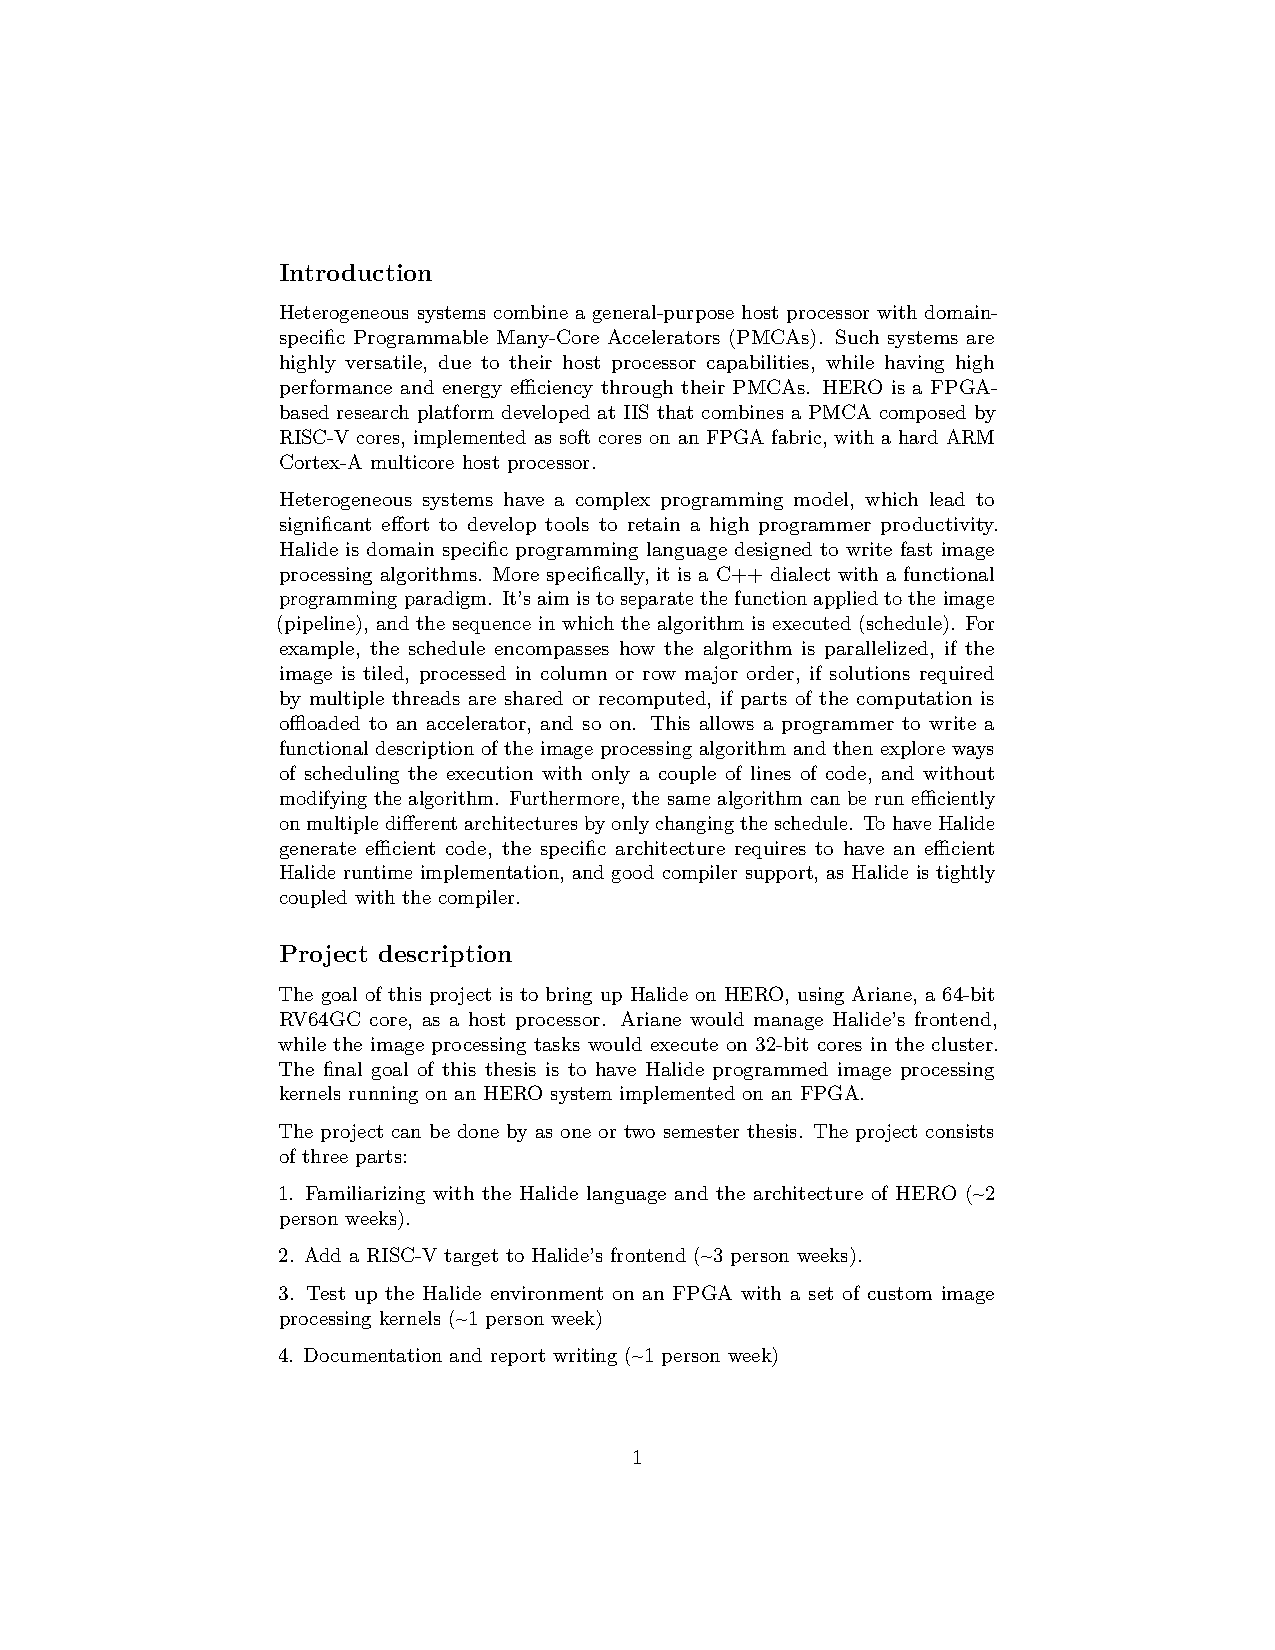
\includepdf[pages=-, turn=false, scale=0.9]{./content/abstract.pdf}
\section{Introduction}

Heterogeneous systems combine a general-purpose host processor with
domain-specific Programmable Many-Core Accelerators (PMCAs). Such
systems are highly versatile, due to their host processor capabilities,
while having high performance and energy efficiency through their PMCAs.
HERO is a FPGA-based research platform developed at IIS that combines a
PMCA composed by RISC-V cores, implemented as soft cores on an FPGA
fabric, with a hard ARM Cortex-A multicore host processor.

Heterogeneous systems have a complex programming model, which lead to
significant effort to develop tools to retain a high programmer
productivity. Halide is domain specific programming language designed to
write fast image processing algorithms. More specifically, it is a C++
dialect with a functional programming paradigm. It's aim is to separate
the function applied to the image (pipeline), and the sequence in which
the algorithm is executed (schedule). For example, the schedule
encompasses how the algorithm is parallelized, if the image is tiled,
processed in column or row major order, if solutions required by
multiple threads are shared or recomputed, if parts of the computation
is offloaded to an accelerator, and so on. This allows a programmer to
write a functional description of the image processing algorithm and
then explore ways of scheduling the execution with only a couple of
lines of code, and without modifying the algorithm. Furthermore, the
same algorithm can be run efficiently on multiple different
architectures by only changing the schedule. To have Halide generate
efficient code, the specific architecture requires to have an efficient
Halide runtime implementation, and good compiler support, as Halide is
tightly coupled with the compiler.

\section{Project description}

The goal of this project is to bring up Halide on HERO, using Ariane, a
64-bit RV64GC core, as a host processor. Ariane would manage Halide's
frontend, while the image processing tasks would execute on 32-bit cores
in the cluster. The final goal of this thesis is to have Halide
programmed image processing kernels running on an HERO system
implemented on an FPGA.

The project can be done by as one or two semester thesis. The project
consists of three parts:

1. Familiarizing with the Halide language and the architecture of HERO
(\textasciitilde2 person weeks).

2. Add a RISC-V target to Halide's frontend (\textasciitilde3 person
weeks).

3. Test up the Halide environment on an FPGA with a set of custom image
processing kernels (\textasciitilde1 person week)

4. Documentation and report writing (\textasciitilde1 person week)

\section{Required skills}

To work on this project, you will need:

\begin{itemize}
\item
  to have worked in the past with at least one RTL language
  (SystemVerilog or Verilog or VHDL). Having followed the VLSI 1 course
  is recommended.
\item
  to have prior knowlegde of the C++ programming language
\item
  to have prior knowledge of hardware design and computer architecture
\item
  to be motivated to work hard on a super cool open-source project
\end{itemize}

\subsubsection{Status: In progress}

\begin{itemize}
\item
  Student: Pierre-Hugues Blelly
\item
  Supervision: \href{:User:Matheusd}{Matheus Cavalcante},
  \href{:User:Sriedel}{Samuel Riedel}, \href{:User:Akurth}{ Andreas
  Kurth}
\end{itemize}

\hypertarget{professor}{%
\subsubsection{Professor}\label{professor}}

\begin{description}
\item[]
\href{http://www.iis.ee.ethz.ch/portrait/staff/lbenini.en.html}{Luca
Benini}
\end{description}

\subsection{Meetings \& Presentations}

The students and advisor(s) agree on weekly meetings to discuss all
relevant decisions and decide on how to proceed. Of course, additional
meetings can be organized to address urgent issues.

Around the middle of the project there is a design review, where senior
members of the lab review your work (bring all the relevant information,
such as prelim. specifications, block diagrams, synthesis reports,
testing strategy, ...) to make sure everything is on track and decide
whether further support is necessary. They also make the definite
decision on whether the chip is actually manufactured (no reason to
worry, if the project is on track) and whether more chip area, a
different package, ... is provided. For more details refer to
\href{http://eda.ee.ethz.ch/index.php/Design_review}{(1)}.

At the end of the project, you have to present/defend your work during a
15 min. presentation and 5 min. of discussion as part of the IIS
Colloquium.

\subsection{References}

\begin{enumerate}
\item
  Andreas Kurth, Pirmin Vogel, Alessandro Capotondi, Andrea Marongiu,
  Luca Benini. HERO: Heterogeneous Embedded Research Platform for
  Exploring RISC-V Manycore Accelerators on FPGA. CARRV' 2017.
  \href{https://doi.org/10.3929/ethz-b-000219249}{link}
\item
  Jonathan Ragan-Kelley, Andrew Adams, Sylvain Paris, Marc Levoy, Saman
  Amarasinghe, Frédo Durand. Decoupling Algorithms from Schedules for
  Easy Optimization of Image Processing Pipelines. SIGGRAPH 2012.
  \href{http://people.csail.mit.edu/jrk/halide12}{link}
\end{enumerate}



\chapter{Declaration of Originality}\label{chap:originality}
Include the declaration of authorship with the \shell{\textbackslash
  includepdf} command (sign it and scan it). For more information
about plagiarism, please visit
\url{https://www.ethz.ch/students/en/studies/performance-assessments/plagiarism.html}

\begin{itemize}
\item \textbf{English version:}
  \url{https://www.ethz.ch/content/dam/ethz/main/education/rechtliches-abschluesse/leistungskontrollen/declaration-originality.pdf}
\item \textbf{German version:}
  \url{https://www.ethz.ch/content/dam/ethz/main/education/rechtliches-abschluesse/leistungskontrollen/plagiat-eigenstaendigkeitserklaerung.pdf}
\end{itemize}

% include the signed declaration of authorship!
\includegraphics[width=.8\textwidth]{./figures/declaration_of_originality.pdf}



%%%%%%%%%%%%%%%%%%%%%%%%%%%%%%%%%%%%%%%%%%%%%%%%%%%%%%%%%%%%%%%%%%%%%%%%
%%%%%%%%%%%%%%%%%%%%%%%%%%%%%%%%%%%%%%%%%%%%%%%%%%%%%%%%%%%%%%%%%%%%%%%
%%%%%                                                                 %
%%%%%     z_02_directories.tex                                        %
%%%%%                                                                 %
%%%%% Author:      Michael Muehlberghuber (<mbgh@iis.ee.ethz.ch>      %
%%%%% Created:     01.07.2012                                         %
%%%%% Description: A description of all files and directories         %
%%%%%              contained within this LaTeX framework.             %
%%%%%                                                                 %
%%%%%                                                                 %
%%%%% History:                                                        %
%%%%%%%%%%%%%%                                                        %
%%%%%                                                                 %
%%%%% 01-Jul-2012 (Michael Muehlberghuber - mbgh@iis.ee.ethz.ch):     %
%%%%% *) Created initial version.                                     %
%%%%%                                                                 %
%%%%%%%%%%%%%%%%%%%%%%%%%%%%%%%%%%%%%%%%%%%%%%%%%%%%%%%%%%%%%%%%%%%%%%%
%%%%%%%%%%%%%%%%%%%%%%%%%%%%%%%%%%%%%%%%%%%%%%%%%%%%%%%%%%%%%%%%%%%%%%%

\chapter{The Template Directory Structure}

This \LaTeX{} framework suitable for creating reports spreads over
various directories and files. In order to give you a short overview
of this structure, the respective directories and the contained files
are described in the following:

\begin{flushleft}
\dirtree{%
.1 /.
  .2 README \DTcomment{README file with a quick start guide.}.
  .2 Makefile \DTcomment{Makefile with some \LaTeX{} related build targets.}.
  .2 report\_template.tex \DTcomment{The main \LaTeX{} file of the report document, which further loads other (content) files.}.
  .2 bib \DTcomment{Contains bibliography related files.}.
    .3 main.bib \DTcomment{Bibliography file.}.
  .2 content \DTcomment{Contains the actual source files of your report.}.
    .3 *$.$tex \DTcomment{Here, multiple content files are provided.}.
  .2 figures \DTcomment{Contains the images which are loaded during your report.}.
    .3 eth\_logo.* \DTcomment{ETH logo in \gls{eps} and \gls{pdf} format.}.
    .3 titlepage\_logo.* \DTcomment{Titlepage logo in \gls{eps} and \gls{pdf} format.}.
    .3 asic\_pinout.* \DTcomment{Sample pinout of an \gls{asic} in \gls{eps} and \gls{pdf} format.}.
  .2 figures\_raw \DTcomment{Contains the raw sources of your figures.}.
    .3 titlepage\_logo.obj \DTcomment{Tgif titlepage logo source.}.
  .2 glossaries \DTcomment{Contains glossaries.}.
    .3 glossaries.tex \DTcomment{The glossaries file containing both the entries of the list of acronym entries and the entries of the main glossary.}.
  .2 preamble \DTcomment{Contains preamble information of the document.}.
    .3 preamble.tex \DTcomment{Preamble of the report document.}.
}
\end{flushleft}


%%% Local Variables: 
%%% mode: latex
%%% TeX-master: "../report_template"
%%% End: 

%%%%%%%%%%%%%%%%%%%%%%%%%%%%%%%%%%%%%%%%%%%%%%%%%%%%%%%%%%%%%%%%%%%%%%%%
%%%%%%%%%%%%%%%%%%%%%%%%%%%%%%%%%%%%%%%%%%%%%%%%%%%%%%%%%%%%%%%%%%%%%%%
%%%%%                                                                 %
%%%%%     z_03_latex_tips.tex                                         %
%%%%%                                                                 %
%%%%% Author:      Michael Muehlberghuber (<mbgh@iis.ee.ethz.ch>      %
%%%%% Created:     01.07.2012                                         %
%%%%% Description: Some LaTeX-specific writing tips                   %
%%%%%                                                                 %
%%%%%                                                                 %
%%%%% History:                                                        %
%%%%%%%%%%%%%%                                                        %
%%%%%                                                                 %
%%%%% 01-Jul-2012 (Michael Muehlberghuber - mbgh@iis.ee.ethz.ch):     %
%%%%% *) Created initial version.                                     %
%%%%%                                                                 %
%%%%%%%%%%%%%%%%%%%%%%%%%%%%%%%%%%%%%%%%%%%%%%%%%%%%%%%%%%%%%%%%%%%%%%%
%%%%%%%%%%%%%%%%%%%%%%%%%%%%%%%%%%%%%%%%%%%%%%%%%%%%%%%%%%%%%%%%%%%%%%%

\chapter{\LaTeX{} Tips}

Writing a report with \LaTeX{} may not be as intuitive as it is the
case with \gls{wysiwyg} editors. Especially if you are using \LaTeX{}
(more or less) the first time, some problems with the syntax will
occur. In general, the present document should already serve as a good
starting point for your report and in the best case you only have to
insert the content of your project based on this framework.

Nevertheless, I will try to give some useful tips with regard to
\LaTeX{} throughout the next sections, which may help you to increase
the quality of your documents even further. If you want to use any of
the presented ideas, simply copy the \LaTeX{} source code of the
appropriate section to your on document and adapt it accordingly.


\section{Compiling a \LaTeX{} Document}
\label{sec:compiling}

Basically, either \shell{latex} or \shell{pdflatex} can be used in
order to generate the document output in \gls{dvi} or \gls{pdf}
format, respectively. Throughout this section I will solely use the
\shell{pdflatex} command for demonstration purposes (if you prefer a
DVI document, just replace the \shell{pdflatex} command by
\shell{latex}0).

Compiling a latex document at the \gls{iis} computers is, in general,
as simple as executing the following command in a UNIX terminal
window:

\begin{shellenv}
pdflatex <document_name>
\end{shellenv}

Currently\footnote{State: July 2012} a \TeX{} Live version from the
year 2008 is the default distribution at the \gls{iis}. In order to
use the present \LaTeX{} framework for your report, you have to use a
more up-to-date version of \TeX{} Live, because the framework uses
some \LaTeX{} packages which are not part of the 2008 version. I
suggest using the 2011 version of \TeX{} Live. The simplest way to
check that you can build the report template successfully, is by
executing:

\begin{shellenv}
pdflatex-2011 report_template.tex
\end{shellenv}

This should (re)generate the \gls{pdf} output of the report template,
i.e., the file you are currently reading through. If typing in the
\shell{-2011} postfix becomes annoying for you, you may add aliases
into your \file{.cshrc} as follows:

\begin{shellenv}
alias latex 'latex-2011'
alias pdflatex 'pdflatex-2011'
\end{shellenv}

If you also want to (re)build the glossaries (maybe you have added
some acronyms or the like), you have to compile your report together
with the glossaries as follows:

\begin{shellenv}
pdflatex-2011 your_report.tex
makeglossaries-2011 your_report
pdflatex-2011 your_report.tex
\end{shellenv}

Furthermore, when you modify the references of your report (within the
bibliography file), you also have to (re)run \textsc{Bib}\TeX{} in
order to update your bibliography, i.e.:

\begin{shellenv}
pdflatex-2011 your_report.tex
bibtex-2011 your_report
pdflatex-2011 your_report.tex
pdflatex-2011 your_report.tex
\end{shellenv}


\section{Figures}
\label{sec:figures}

In order to include an image into your report (as it has been done
within in the previous sample chapters), you may use the
\texttt{figure} floating environment. With that, \LaTeX{} will take
care of placing them nicely and you can focus on the actual content of
your document. Figure~\ref{fig:std_eth_logo} shows an example of how
to insert a single figure.

\begin{figure}[htbp]
 \centering\includegraphics[width=0.4\linewidth]{./figures/eth_logo}
 \caption{Standard ETH logo.}
 \label{fig:std_eth_logo}
\end{figure}

If you want to place multiple figures side-by-side, you can do this
with the use of \texttt{minipages}. Figure~\ref{fig:left_eth_logo} and
\ref{fig:right_eth_logo} illustrates an example.

\begin{figure}[htbp]
 \begin{minipage}[t]{0.45\linewidth}
  \centering\includegraphics[width=1.0\linewidth]{./figures/eth_logo}
  \caption{Left ETH logo.}
  \label{fig:left_eth_logo}
 \end{minipage}\hfill
 \begin{minipage}[t]{0.45\linewidth}
  \centering\includegraphics[width=1.0\linewidth]{./figures/eth_logo}
  \caption{Right ETH logo.}
  \label{fig:right_eth_logo}
 \end{minipage}
\end{figure}

In order to create a single figure with multiple subfigures, you can
do this as presented in Figure~\ref{fig:eth_logo_sub}

\begin{figure}[htbp]
 \centering
 \subfloat[Left ETH logo.]{\includegraphics[width=0.3\textwidth]{./figures/eth_logo}}\hfill
 \subfloat[Center ETH logo.]{\includegraphics[width=0.3\textwidth]{./figures/eth_logo}}\hfill
 \subfloat[Right ETH logo.]{\includegraphics[width=0.3\textwidth]{./figures/eth_logo}}
 \caption{Multiple ETH logos as subfigures.}
 \label{fig:eth_logo_sub}
\end{figure}


\section{Tables}
\label{sec:tables}

Tables in \LaTeX{} allow you to present your results quite
nicely. Table~\ref{tab:std_table} shows a standard table.

\begin{table}[htbp]
 \caption{Standard table.}
 \label{tab:std_table}
 \centering\begin{tabular}{@{}lcr@{}} \toprule
  \textbf{Row 1 - Column 1} & \textbf{Row 1 - Column 2} & \textbf{Row 1 - Column 3} \\ \midrule
  Row 2 - Column 1 & Row 2 - Column 2 & Row 2 - Column 3 \\
  Row 3 - Column 1 & Row 3 - Column 2 & Row 3 - Column 3 \\
  Row 4 - Column 1 & Row 4 - Column 2 & Row 4 - Column 3 \\ \bottomrule
 \end{tabular}
\end{table}

Sometimes you may want to add a table which stretches one of its
columns in order to reach the full width of the document. Such an
example is shown in Table~\ref{tab:stretched_table}.

\begin{table}[htbp]
 \caption{Stretched table.}
 \label{tab:stretched_table}
 \centering\begin{tabularx}{1.0\linewidth}{@{}Xcr@{}} \toprule
  \textbf{Row 1 - Column 1} & \textbf{Row 1 - Column 2} & \textbf{Row 1 - Column 3} \\ \midrule
  Row 2 - Column 1 & Row 2 - Column 2 & Row 2 - Column 3 \\
  Row 3 - Column 1 & Row 3 - Column 2 & Row 3 - Column 3 \\
  Row 4 - Column 1 & Row 4 - Column 2 & Row 4 - Column 3 \\ \bottomrule
 \end{tabularx}
\end{table}

If you need to place two tables next to each other, you may use an
approach based on \texttt{minipages} as shown in Table~\ref{tbl:left}
and Table~\ref{tbl:right}.

\begin{figure}
  \begin{minipage}{0.49\textwidth}
    \captionof{table}{Left table.}
    \label{tbl:left}
    \centering\begin{tabular}{@{}lr@{}} \toprule
      Row 1 - Column 1 & Row 1 - Column 2 \\ \midrule
      Row 2 - Column 1 & Row 2 - Column 2 \\
      Row 3 - Column 1 & Row 3 - Column 2 \\
      Row 4 - Column 1 & Row 4 - Column 2 \\ \bottomrule
    \end{tabular}
  \end{minipage} \hfill
  %
  \begin{minipage}{0.49\textwidth}
    \captionof{table}{Right table.}
    \label{tbl:right}
    \centering\begin{tabular}{@{}lr@{}} \toprule
      Row 1 - Column 1 & Row 1 - Column 2 \\ \midrule
      Row 2 - Column 1 & Row 2 - Column 2 \\
      Row 3 - Column 1 & Row 3 - Column 2 \\
      Row 4 - Column 1 & Row 4 - Column 2 \\ \bottomrule
    \end{tabular}
  \end{minipage}
\end{figure}

\section{Creating Glossaries}

In order to generate a glossary within your report (e.g., a list of
acronyms or an actual glossary), take a look into the file
\texttt{glossaries.tex}. There, you will find some examples on how to
define an acronym as well as a glossary entry. If you want to
reference one of the acronyms within your report, you can do it the
same way as I did it with the \gls{led} right here (just take a look
into the source code).

As already mentioned in Section~\ref{sec:compiling}, you have to
rebuild your glossaries in order to display changes. For that, you
first have to build your document using \texttt{latex-2011} or
\texttt{pdflatex-2011} in a shell window, or the \textit{build-button}
in your preferred \LaTeX{} editor GUI. Next, you have to call
\texttt{makeglossaries-2011 \parameter{file\_name}} in a shell
window\footnote{The \texttt{makeglossaries} script is a Perl script
  available at the IIS computer system and should also be part of most
  \TeX{} distributions.}, followed by another build process of your
main source file, i.e.:

\begin{shellenv}
pdflatex-2011 your_report.tex
makeglossaries-2011 your_report
pdflatex-2011 your_report.tex
\end{shellenv}


\section{Creating Algorithm Boxes}

Algorithm boxes in \LaTeX{} allow you to present your algorithms in
pseudo code as shown in the following example:

\begin{algorithm}
  \SetKwData{Left}{left}\SetKwData{This}{this}\SetKwData{Up}{up}
  \SetKwFunction{Union}{Union}\SetKwFunction{FindCompress}{FindCompress}
  \SetKwInOut{Input}{input}\SetKwInOut{Output}{output}

  \Input{A bitmap $Im$ of size $w\times l$}
  \Output{A partition of the bitmap}
  \BlankLine
  \emph{special treatment of the first line}\;
  \For{$i\leftarrow 2$ \KwTo $l$}{
    \emph{special treatment of the first element of line $i$}\;
    \For{$j\leftarrow 2$ \KwTo $w$}{\label{forins}
      \Left$\leftarrow$ \FindCompress{$Im[i,j-1]$}\;
      \Up$\leftarrow$ \FindCompress{$Im[i-1,]$}\;
      \This$\leftarrow$ \FindCompress{$Im[i,j]$}\;
      \If(\tcp*[h]{O(\Left,\This)==1}){\Left compatible with \This}{\label{lt}
        \lIf{\Left $<$ \This}{\Union{\Left,\This}}\;
        \lElse{\Union{\This,\Left}\;}
      }
      \If(\tcp*[f]{O(\Up,\This)==1}){\Up compatible with \This}{\label{ut}
        \lIf{\Up $<$ \This}{\Union{\Up,\This}}\;
        \tcp{\This is put under \Up to keep tree as flat as possible}\label{cmt}
        \lElse{\Union{\This,\Up}}\tcp*[r]{\This linked to \Up}\label{lelse}
      }
    }
    \lForEach{element $e$ of the line $i$}{\FindCompress{p}}
  }
  \caption{disjoint decomposition}\label{algo_disjdecomp}
\end{algorithm}


% \section{Citing}


% \section{Units}

%%% Local Variables:
%%% mode: latex
%%% TeX-master: "../report_template"
%%% End:

%%%%%%%%%%%%%%%%%%%%%%%%%%%%%%%%%%%%%%%%%%%%%%%%%%%%%%%%%%%%%%%%%%%%%%%%
%%%%%%%%%%%%%%%%%%%%%%%%%%%%%%%%%%%%%%%%%%%%%%%%%%%%%%%%%%%%%%%%%%%%%%%
%%%%%                                                                 %
%%%%%     z_04_writing_tips.tex                                       %
%%%%%                                                                 %
%%%%% Author:      Michael Muehlberghuber (<mbgh@iis.ee.ethz.ch>      %
%%%%% Created:     01.07.2012                                         %
%%%%% Description: Some Writing-specific tips in general.             %
%%%%%                                                                 %
%%%%% History:                                                        %
%%%%%%%%%%%%%%                                                        %
%%%%%                                                                 %
%%%%% 01-Jul-2012 (Michael Muehlberghuber - mbgh@iis.ee.ethz.ch):     %
%%%%% *) Created initial version.                                     %
%%%%%                                                                 %
%%%%%%%%%%%%%%%%%%%%%%%%%%%%%%%%%%%%%%%%%%%%%%%%%%%%%%%%%%%%%%%%%%%%%%%
%%%%%%%%%%%%%%%%%%%%%%%%%%%%%%%%%%%%%%%%%%%%%%%%%%%%%%%%%%%%%%%%%%%%%%%

\chapter{General Writing Guidelines}

As soon as you get familiar with the syntax of \LaTeX{} (and I can
promise you, you will get familiar with it quite quickly as soon as
you start writing your reports with \LaTeX{}), some more general
writing tips might become of interest for your. Therefore, I collected
a few general writing guidlines in the following sections, some of
them with regard to \LaTeX{}, some of them not.

\paragraph{Placement of Floating Environments}
Figures and tables are the two most prominent examples for floating
environments. Although the figure examples presented in
Section~\ref{sec:figures} use \texttt{[htbp]} to tell \LaTeX{} how to
place them, you should normally only use the \texttt{h} parameter if
you really require it. Since \LaTeX{} then at first tries to place the
figure at the same position as its source code, this somehow
contradicts with the actual purpose of the \texttt{figure}
environment. So, in general, try to place floating environments using
one of the following parameters:

\begin{description}
\item[t] Place the floating environment on \textbf{t}op of a page.
\item[b] Place the floating environment on the \textbf{b}ottom of a
  page.
\item[p] Puts the floating environment on a single \textit{floating
    \textbf{p}age} with other floating environments.
\end{description}


\paragraph{Positioning of Figure and Table Captions}
Captions of figures are, in general, placed below the actual figure,
whereas captions of tables should be placed on top of
them. Section~\ref{sec:figures} and \ref{sec:tables} contain some
examples for figures and tables, including correct placement of
captions.


\paragraph{Avoid Unneccessary \LaTeX{} Packages}
Although there are so many ``cool'' \LaTeX{} packages available
everywhere on the Internet, try to use only those, which you really
require. The main problem with loading too many, more or less unknown,
packages is that some of them might redefine some commands, etc.,
which are used by another package which asumes that command to be the
original one. Keeping track of these changes and the relations between
different packages, is quite annoying and takes quite a lot of
time. Hence, keep your preamble simple with regard to packages.


\paragraph{Make Use of Vector Drawings}
Since \LaTeX{} handles vector drawings pretty good and their
scalability allows you to print them in any resolution, prefer them
compared to their pixel counterparts and use them whenever possible.

% \paragraph{Equations Within the ``Text-Flow''}

% \paragraph{Punctuation within Captions}
% \begin{itemize}
%  \item No second fullstop when ending sentences with abbreviations like
%  etc.
% \end{itemize}

%%% Local Variables:
%%% mode: latex
%%% TeX-master: "../report_template"
%%% End:


\backmatter

% Print the main glossary.
\printglossary[type=main,title=Glossary]


% Print the bibliography.
\nocite*{} % Print non-cited references as well.
\bibliographystyle{IEEEtran}
\bibliography{IEEEabrv,./bib/main.bib}


\end{document}
%%%%%%%%%%%%%%%%%%%%%%%%%%%%%%%%%%%%%%%%%%%%%%%%%%%%%%%%%%%%%%%%%%%%%%%
%%%%%                                                                 %
%%%%%     End of Document                                             %
%%%%%                                                                 %
%%%%%%%%%%%%%%%%%%%%%%%%%%%%%%%%%%%%%%%%%%%%%%%%%%%%%%%%%%%%%%%%%%%%%%%
